\documentclass[letterpaper, 12pt]{article}
\usepackage[margin=1in]{geometry}
\usepackage{amsmath}
\usepackage{amssymb}
\usepackage{fancyhdr}
%\usepackage{hyperref}
%\usepackage{xcolor}
\setlength{\headheight}{15pt}
\usepackage{tikz}
\usetikzlibrary{positioning, calc}

\pagestyle{fancy}
\fancyhf{}

\rhead{
    Shengdong Li
    Calc 1
}
\rfoot{
    page \thepage
}

\usepackage{indentfirst}

\begin{document}
\title{Concluding Lesson}
\author{by Shengdong Li}
\date{17 May 2020}
\maketitle

\section{Intro}
Hello everyone, since it seemed to me that the initial reception for the video lesson was quite nice, I figured that perhaps a written lesson would accompany it quite well for the conclusion, with a better formatting of steps and cleaner text.

\section{Solving the Integral of $\int_{ }^{ }\frac{x^{2}}{\sqrt{4-x^{2}}}dx$}
\subsection{Why do we substitute $x$ for trig functions}
\begin{align}
    \intertext{The standard values for substitution are derived as follows, with the goal of turning a costant and a sinusoid into just a sinusoid, so they can be taken from under the square root.}
    \sin^{2}\theta+\cos^{2}\theta&=1
    \intertext{Moving $\sin$ to the right gives}
    \cos^{2}\theta&=1-\sin^{2}\theta
    \intertext{Which the right side is in the form of $a^{2}-x^{2}$. Next, dividing the original identity by $\cos$ gives...}
    \frac{\sin^{2}\theta}{\cos^{2}\theta}+\frac{\cos^{2}\theta}{\cos^{2}\theta}&=\frac{1}{\cos^{2}\theta}\\
    \tan^{2}\theta+1&=\sec^{2}\theta
    \intertext{Which the left side is in the form of $x^{2}+a^{2}$. Finally, moving $1$ to the right gives}
    \tan^{2}\theta&=\sec^{2}\theta-1
    \intertext{In which the right side is in the form of $x^{2}-a^{2}$. Therefore, we now know the values that we should substitute for $x$ when we see a certain function under the parenthesis.}
\end{align}
\subsection{What to actually substitute for trig functions}
\begin{align}
    \intertext{When presented with }
    &a^{2}-x^{2}
    \intertext{We substitute }
    x&=a\sin\theta
    \intertext{To get}
    &\cos\theta
    \intertext{When presented with }
&x^{2}+a^{2}
    \intertext{We substitute }
x&=a\tan\theta
    \intertext{To get}
&\sec\theta
    \intertext{When presented with }
&x^{2}-a^{2}
    \intertext{We substitute }
x&=a\sec\theta
    \intertext{To get}
&\tan\theta
\end{align}
\subsection{Onto the integral at hand}
$$
\int_{ }^{ }\frac{x^{2}}{\sqrt{4-x^{2}}}dx
$$
\begin{align}
    \intertext{As we can see, $4-x^2$ is in the form of $a^2-x^2$, which calls for}
    x&=a\sin\theta\\
    a^{2}&=4\\
    a&=2\\
    \intertext{And therefore,}
    x&=2\sin\theta
    \intertext{Don't forget that trig-sub is just like $u$-sub, you have to account for $dx$ and put it in terms of $\theta$}
    dx&=2\cos\theta d\theta
    \intertext{Now we plugin!}
    \int_{ }^{ }\frac{x^{2}}{\sqrt{4-x^{2}}}dx&=\int_{ }^{ }\frac{\left(2\sin\theta\right)^{2}2\cos\theta d\theta}{\sqrt{4-\left(2\sin\theta\right)^{2}}}
    \intertext{Let's work on the bottom square root first. }
    \sqrt{4-\left(2\sin\theta\right)^{2}}&=\sqrt{4-4\sin^{2}\theta}
    \intertext{We can factor out the $4$}
    &=\sqrt{4\left(1-\sin^{2}\theta\right)}
    \intertext{Which, recall earlier, that we substitute $\sin$ just so that we can use the identity to get $\cos$}
    &=\sqrt{4\cos^{2}\theta}\\
    &=2\cos\theta
    \intertext{Now back to the main function, this results in}
    &=\int_{ }^{ }\frac{\left(2\sin\theta\right)^{2}2\cos\theta d\theta}{2\cos\theta}
    \intertext{In which the cosines cancel, and we can simplify a bit}
    &=\int_{ }^{ }\left(2\sin\theta\right)^{2}d\theta\\
    &=\int_{ }^{ }4\sin^{2}\theta d\theta\\
    &=4\int_{ }^{ }\sin^{2}\theta d\theta
    \intertext{Here, it's really hard to progress, without knowing a half angle identity:}
    \sin^{2}\theta&=\frac{1-\cos2\theta}{2}
    \intertext{It's a pretty straightforward solve for the integral from there.}
    &=4\int_{ }^{ }\frac{1-\cos2\theta}{2}d\theta\\
    &=2\int_{ }^{ }d\theta-2\int_{ }^{ }\cos2\theta d\theta\\
    &=2\theta-2\int_{ }^{ }\cos2\theta d\theta
    \intertext{Here we can $u$-sub to integrate the cosine function}
u&=2\theta\\
du&=2d\theta\\
\frac{1}{2}du&=d\theta\\
&=2\theta-\int_{ }^{ }\cos udu\\
&=2\theta-\sin u\\
&=2\theta-\sin2\theta
\intertext{Now we have to put $\theta$ back in terms of $x$. Recall the value that we substituted for $x$ earlier...}
x&=2\sin\theta
\intertext{To get $\theta$, we just have to use $\arcsin$}
\frac{x}{2}&=\sin\theta\\
\sin^{-1}\left(\frac{x}{2}\right)&=\theta\\
2\theta&=2\sin^{-1}\left(\frac{x}{2}\right)
\intertext{Now putting $\sin 2\theta$ in terms of $x$ is a bit harder. We can first the double-angle identity of}
\sin2\theta&=2\sin\theta\cos\theta
\intertext{Which takes care of the $\sin x$}
&=2\left(\frac{x}{2}\right)\cos\theta\\
&=x\cos\theta
\intertext{But what about the $\cos\theta$? To solve this, we have to draw a triangle. We know that $\frac{x}{2}=\sin\theta$...}
\end{align}
\begin{center}
    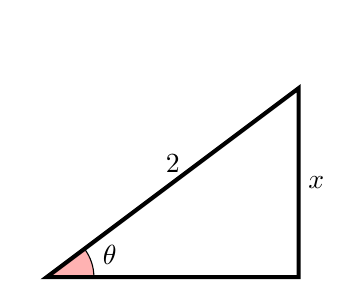
\begin{tikzpicture}[scale=0.8]
        % draw the background
        %\draw [line width=1.5pt, fill=gray!2] (0,0) -- (60:4) -- (4,0) -- cycle;

        \coordinate[label=left:$$]  (A) at (0,0);
        \coordinate[label=right:$$] (B) at (4,0);
        \coordinate[label=above:$$] (C) at (4,3);

        \coordinate[label=below:$$](c) at ($ (A)!.5!(B) $);
        \coordinate[label=above:$2$](b) at ($ (A)!.5!(C) $);
        \coordinate[label=right:$x$](a) at ($ (B)!.5!(C) $);

        %angle alpha
        \draw[fill=red!30] (0,0) -- (0:0.75cm) arc (0:36.87:.75cm);
        \draw (1cm,0.35cm) node {$\theta$};

        % angle beta
        %\begin{scope}[shift={(4cm,0cm)}]
        %    \draw[fill=green!30] (0,0) -- (-180:0.75cm) arc (180:120:0.75cm);
        %    \draw (150:0.5cm) node {$\beta$};
        %\end{scope}

        % angle gamma
        %\begin{scope}[shift={(60:4)}]
        %    \draw[fill=green!30] (0,0) -- (-120:.75cm) arc (-120:-60:.75cm);
        %    \draw (-90:0.5cm) node {$\gamma$};
        %\end{scope}

        % the triangle
        \draw [line width=1.5pt] (A) -- (B) -- (C) -- cycle;
    \end{tikzpicture}
\end{center}
Now we just solve for the missing side using the pythagorean theorem!
\begin{align}
    b^2&=2^2-x^2\\
    b&=\sqrt{4-x^2}
\end{align}
Which gives us a completed triangle.
\begin{center}
    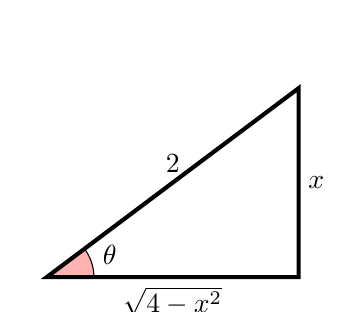
\begin{tikzpicture}[scale=0.8]
        % draw the background
        %\draw [line width=1.5pt, fill=gray!2] (0,0) -- (60:4) -- (4,0) -- cycle;

        \coordinate[label=left:$$]  (A) at (0,0);
        \coordinate[label=right:$$] (B) at (4,0);
        \coordinate[label=above:$$] (C) at (4,3);

        \coordinate[label=below:$\sqrt{4-x^2}$](c) at ($ (A)!.5!(B) $);
        \coordinate[label=above:$2$](b) at ($ (A)!.5!(C) $);
        \coordinate[label=right:$x$](a) at ($ (B)!.5!(C) $);

        %angle alpha
        \draw[fill=red!30] (0,0) -- (0:0.75cm) arc (0:36.87:.75cm);
        \draw (1cm,0.35cm) node {$\theta$};

        % angle beta
        %\begin{scope}[shift={(4cm,0cm)}]
        %    \draw[fill=green!30] (0,0) -- (-180:0.75cm) arc (180:120:0.75cm);
        %    \draw (150:0.5cm) node {$\beta$};
        %\end{scope}

        % angle gamma
        %\begin{scope}[shift={(60:4)}]
        %    \draw[fill=green!30] (0,0) -- (-120:.75cm) arc (-120:-60:.75cm);
        %    \draw (-90:0.5cm) node {$\gamma$};
        %\end{scope}

        % the triangle
        \draw [line width=1.5pt] (A) -- (B) -- (C) -- cycle;
    \end{tikzpicture}
\end{center}
\begin{align}
    \intertext{Now, $\cos$ is $\frac{Adjacent}{Hypotenuse}$. Evaluating this based off of the sides of the triangle gives}
    \cos\theta&=\frac{\sqrt{4-x^{2}}}{2}
    \intertext{Which, recall earlier that}
    \sin2\theta&=x\cos\theta
    \intertext{Which now equal}
    &=\frac{x\sqrt{4-x^{2}}}{2}
    \intertext{Making our final answer}
    &=\boxed{2\sin^{-1}\left(\frac{x}{2}\right)-\frac{x\sqrt{4-x^{2}}}{2}+C}
\end{align}
\section{Solving the integral of}
$$
\int_{ }^{ }\frac{1}{x^{3}\sqrt{x^{2}-9}}dx
$$
\begin{align}
    \intertext{As we can see, $x^{2}-9$ is clearly in the form of $x^{2}-a^{2}$, which calls for}
    x&=a\sec\theta\\
    a^{2}&=9\\
    a&=3
    \intertext{And therefore,}
    x&=3\sec\theta\\
    dx&=3\sec\theta\tan\theta d\theta
    \intertext{Now plugin!}
    \int_{ }^{ }\frac{1}{x^{3}\sqrt{x^{2}-9}}dx&=\int_{ }^{ }\frac{3\sec\theta\tan\theta d\theta}{\left(3\sec\theta\right)^{3}\sqrt{\left(3\sec\theta\right)^{2}-9}}
    \intertext{Let's work on the square root first}
    \sqrt{\left(3\sec\theta\right)^{2}-9}&=\sqrt{9\sec^{2}\theta-9}
    \intertext{We can factor out the $9$}
    &=\sqrt{9\left(\sec^{2}\theta-1\right)}
    \intertext{Recall that $\sec^{2}\theta-1$ is the trig identity that we're going for when subbing in $\sec$}
    &=\sqrt{9\tan^{2}\theta}\\
    &=3\tan\theta
    \intertext{Now back to the main integral!}
    &=\int_{ }^{ }\frac{3\sec\theta\tan\theta d\theta}{\left(3\sec\theta\right)^{3}\cdot3\tan\theta}
    \intertext{We see that the $\sec$ and $\tan$ cancel}
    &=\int_{ }^{ }\frac{d\theta}{\left(3\sec\theta\right)^{2}\cdot3}
    \intertext{Let's mulitply out and distribute factors}
    &=\int_{ }^{ }\frac{d\theta}{27\sec^{2}\theta}\\
    &=\frac{1}{27}\int_{ }^{ }\frac{d\theta}{\sec^{2}\theta}
    \intertext{Recall that $\sec\theta=\frac{1}{\cos\theta}$}
    &=\frac{1}{27}\int_{ }^{ }\frac{d\theta}{\left(\frac{1}{\cos^{2}\theta}\right)}\\
    &=\frac{1}{27}\int_{ }^{ }\cos^{2}\theta d\theta
    \intertext{And now, similar to the integral that we solved earlier, we can use a half angle identity here}
    \cos^{2}\theta&=\frac{1+\cos2\theta}{2}
    \intertext{Pluggin that into the integral gives}
    &=\frac{1}{27}\int_{ }^{ }\frac{1+\cos2\theta}{2}d\theta
    \intertext{Which we can solve pretty standardly}
    &=\frac{1}{54}\int_{ }^{ }1+\cos2\theta d\theta\\
    &=\frac{1}{54}\int_{ }^{ }d\theta+\frac{1}{54}\int_{ }^{ }\cos2\theta d\theta\\
    &=\frac{1}{54}\theta+\frac{1}{54}\int_{ }^{ }\cos2\theta d\theta\\
u&=2\theta\\
du&=2d\theta\\
\frac{1}{2}du&=d\theta\\
&=\frac{1}{54}\theta+\frac{1}{108}\int_{ }^{ }\cos udu\\
&=\frac{1}{54}\theta+\frac{1}{108}\sin u\\
&=\frac{1}{54}\theta+\frac{1}{108}\sin2\theta
\intertext{Let's use the double-angle identity again}
\sin2\theta&=2\sin\theta\cos\theta\\
&=\frac{1}{54}\theta+\frac{1}{54}\sin\theta\cos\theta
\intertext{Recall the value of $x$ that we defined earlier}
x&=3\sec\theta
\intertext{Which means that}
\frac{x}{3}&=\sec\theta
\intertext{And...}
\frac{3}{x}&=\cos\theta
\intertext{We can use $\sec^{-1}$ to get $\theta$}
\sec^{-1}\left(\frac{x}{3}\right)&=\theta
\end{align}
But to get $\sin$, we have to draw a triangle again, with $\cos\theta=\frac{3}{x}$ in mind.
\begin{center}
    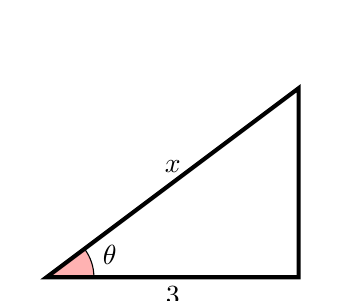
\begin{tikzpicture}[scale=0.8]
        % draw the background
        %\draw [line width=1.5pt, fill=gray!2] (0,0) -- (60:4) -- (4,0) -- cycle;

        \coordinate[label=left:$$]  (A) at (0,0);
        \coordinate[label=right:$$] (B) at (4,0);
        \coordinate[label=above:$$] (C) at (4,3);

        \coordinate[label=below:$3$](c) at ($ (A)!.5!(B) $);
        \coordinate[label=above:$x$](b) at ($ (A)!.5!(C) $);
        \coordinate[label=right:$$](a) at ($ (B)!.5!(C) $);

        %angle alpha
        \draw[fill=red!30] (0,0) -- (0:0.75cm) arc (0:36.87:.75cm);
        \draw (1cm,0.35cm) node {$\theta$};

        % angle beta
        %\begin{scope}[shift={(4cm,0cm)}]
        %    \draw[fill=green!30] (0,0) -- (-180:0.75cm) arc (180:120:0.75cm);
        %    \draw (150:0.5cm) node {$\beta$};
        %\end{scope}

        % angle gamma
        %\begin{scope}[shift={(60:4)}]
        %    \draw[fill=green!30] (0,0) -- (-120:.75cm) arc (-120:-60:.75cm);
        %    \draw (-90:0.5cm) node {$\gamma$};
        %\end{scope}

        % the triangle
        \draw [line width=1.5pt] (A) -- (B) -- (C) -- cycle;
    \end{tikzpicture}
\end{center}
\begin{align}
    \intertext{Using the pythagorean theorem,}
    b^{2}&=x^{2}-3^{2}\\
    b&=\sqrt{x^{2}-9}
\end{align}
\begin{center}
    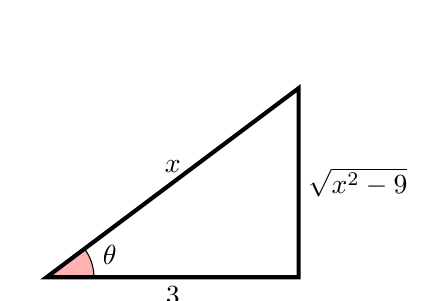
\begin{tikzpicture}[scale=0.8]
        % draw the background
        %\draw [line width=1.5pt, fill=gray!2] (0,0) -- (60:4) -- (4,0) -- cycle;

        \coordinate[label=left:$$]  (A) at (0,0);
        \coordinate[label=right:$$] (B) at (4,0);
        \coordinate[label=above:$$] (C) at (4,3);

        \coordinate[label=below:$3$](c) at ($ (A)!.5!(B) $);
        \coordinate[label=above:$x$](b) at ($ (A)!.5!(C) $);
        \coordinate[label=right:$\sqrt{x^{2}-9}$](a) at ($ (B)!.5!(C) $);

        %angle alpha
        \draw[fill=red!30] (0,0) -- (0:0.75cm) arc (0:36.87:.75cm);
        \draw (1cm,0.35cm) node {$\theta$};

        % angle beta
        %\begin{scope}[shift={(4cm,0cm)}]
        %    \draw[fill=green!30] (0,0) -- (-180:0.75cm) arc (180:120:0.75cm);
        %    \draw (150:0.5cm) node {$\beta$};
        %\end{scope}

        % angle gamma
        %\begin{scope}[shift={(60:4)}]
        %    \draw[fill=green!30] (0,0) -- (-120:.75cm) arc (-120:-60:.75cm);
        %    \draw (-90:0.5cm) node {$\gamma$};
        %\end{scope}

        % the triangle
        \draw [line width=1.5pt] (A) -- (B) -- (C) -- cycle;
    \end{tikzpicture}
\end{center}
\begin{align}
    \intertext{So our $\sin$ value derived from the graph is}
    \sin\theta&=\frac{\sqrt{x^{2}-9}}{x}
    \intertext{Now we can plugin all of these values into our expression that we had.}
    \frac{1}{54}\theta+\frac{1}{54}\sin\theta\cos\theta&=\frac{1}{54}\sec^{-1}\left(\frac{x}{3}\right)+\frac{1}{54}\cdot\frac{3}{x}\cdot\sqrt{x^{2}-9}\\
    &=\boxed{
\frac{1}{54}\sec^{-1}\left(\frac{x}{3}\right)+\frac{1}{18}\frac{\sqrt{x^{2}-9}}{x}+C}
\end{align}
\end{document}